\begin{figure}[t]
\centering
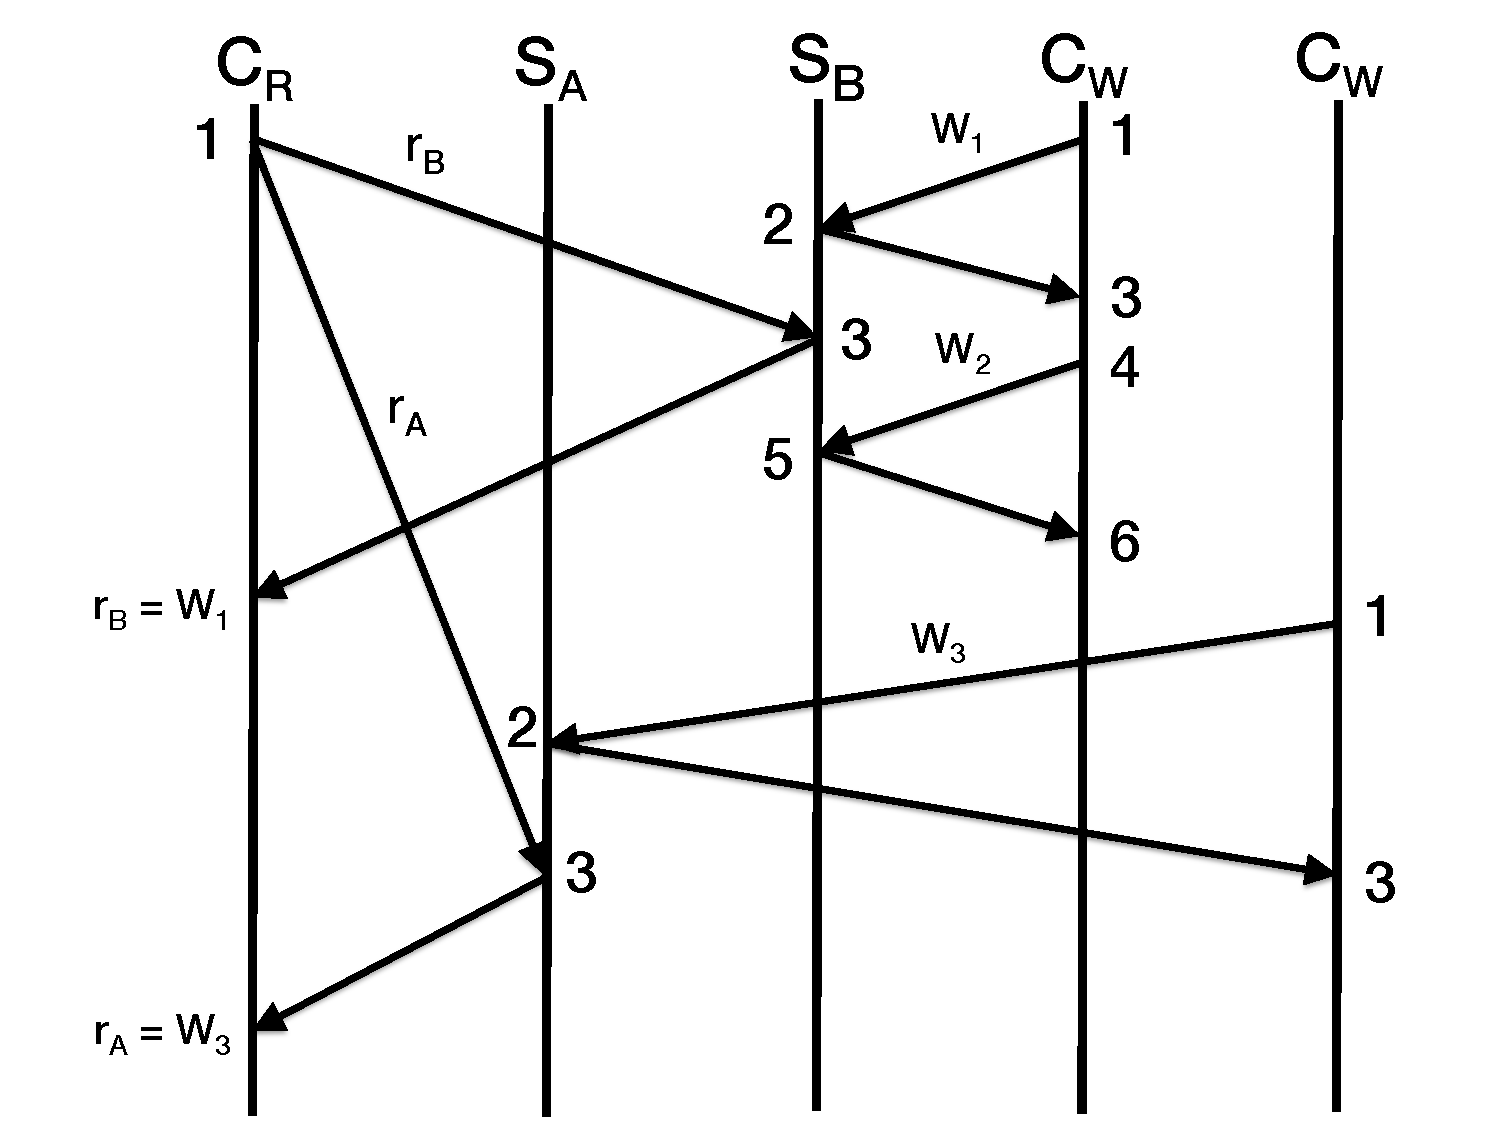
\includegraphics[width=1.0\columnwidth]{figures/eiger-example-2.pdf}
\caption{An example execution that shows Eiger's \textsc{READ} transaction algorithm is not strictly serializable. $w_1$, $w_2$, and $w_3$ are three writes, where $w_3$ is issued after $w_2$ finishes. $r_A$ and $r_B$ are read operations from the same \textsc{READ} transaction $R$, which is concurrent with all three writes. Each number is a value of the logical clock on the machine (process) as a result of message exchange.}
\label{fig:eigerrot}
\end{figure}


\section{Eiger's \rots{} are not Strictly Serializable}
\label{app:eiger_not_s}
%\label{sec:eigerrot}
Eiger~\cite{Lloyd:nsdi2013} targeted a geo-replicated setting, which provided causal consistency across wide areas with fast \textsc{READ} and \textsc{WRITE} transactions handled by each datacenter locally. While not focusing on making transactions strictly serializable, Eiger made a claim that its \textsc{READ} transactions within the local datacenter were strictly serializable. Thus, in SNOW, there was a claim that Eiger was the only system, which had bounded latency while providing the strongest guarantees, and the practical lower bound for property $O$ in existing SNW algorithms was three because Eiger's \textsc{READ} transactions required at most three rounds, i.e., the fewest in all examined existing work, were non-blocking, compatible with \textsc{WRITE} transactions, and were claimed to be strictly serializable. In this section, we correct this claim to be that there was no algorithm, which had bounded latency while providing the strongest guarantees by proving that Eiger's \textsc{READ} transactions are not strictly serializable. In Section~\ref{mwmr_snow_one_version, mwmr_snow_one_round, mwmr_snow_one_round}, we provide the first set of novel SNW algorithms that have bounded latency and prove they are correct.

The insight on why Eiger's \textsc{READ} transactions are not strictly serializable is that Eiger uses logical timestamps, i.e., Lamport clocks, to track the ordering of operations, and logical clocks are not able to identify the real-time ordering between operations that do not have causal relationship, i.e., operations from different processes. Strict serializability, however, requires the real-time ordering to be respected.

Figure~\ref{fig:eigerrot} is an example execution, which is allowed by Eiger but violates strict serializability. 
%$S_A$ and $S_B$ are two servers with initial values $old$. $w_1$ is a write operation that updates $S_A$ with value $new$. After $w_1$ finishes, $w_2$ is issued by another client different from the one who issued $w_1$, and updates $S_B$ with value $new$. Because $w_2$ starts after $w_1$ finishes, $w_2$ should be ordered after $w_1$ by the real-time ordering requirement of strict serializability, i.e., if a READ transaction sees $w_2$, it has to also observe the effect of $w_1$. Because $w_1$ and $w_2$ are from different clients and they do not have causal relationship, it is possible for $w_1$ to commit at the larger logical time than $w_2$, e.g., 10 as shown in Figure~\ref{fig:eigerrot}. $r_1$ and $r_2$ are from the same READ transaction and return $old$ from $S_A$ and $new$ from $S_B$. Because of the misordered logical timestamps, the result is acceptable to Eiger's READ transaction algorithm, but the result violates strict serializability because the READ transaction sees $w_2$ but not $w_1$.
Real time goes downwards in the diagram. Each number is a value of the Lamport clock on the machine (process) as a result of message exchange. Initially all processes have Lamport clock value $0$, and no messages happened before the execution in Figure~\ref{fig:eigerrot}. A \textsc{READ} transaction $R=\{r_A, r_B\}$ reads values on $S_A$ and $S_B$ respectively. Due to the asynchronous nature of the network, $r_B$ arrives on $S_B$ before $w_2$ and $r_A$ arrives after $w_3$. Following the \textsc{READ} transaction algorithm of Eiger, $r_A$ returns the value of $w_3$ and its valid logical duration, i.e., $[2,3]$. Similarly, $r_B$ returns the value of $w_1$ and its valid logical duration, i.e., $[2,3]$. Because the two logical durations overlap, Eiger claims the combined values of $r_A$ and $r_B$ are consistent and accept them. However, because $w_3$ starts after $w_2$ finishes, $w_3$ is in real time after $w_2$. By strict serializability, if a \textsc{READ} transaction sees the value of $w_3$, then it has to also observe the effect of $w_2$. Hence, $R$, which returns the values of $w_1$ and $w_3$, violates strict serializability.
